% Stage 3 report: transient calibration, the transient predictor, the final models and their
% validation on generated floorplans, robustness, and the tool.
% Compile from this folder: pdflatex stage3.tex (twice).
\documentclass[11pt,a4paper]{article}
\usepackage[margin=2.2cm]{geometry}
\usepackage[T1]{fontenc}
\usepackage{lmodern}
\usepackage{amsmath}
\usepackage{graphicx}
\usepackage{booktabs}
\usepackage{array}
\usepackage{enumitem}
\usepackage{xcolor}
\usepackage{caption}
\usepackage{float}
\usepackage[section]{placeins}
\usepackage[hidelinks]{hyperref}
\graphicspath{{../../experiments/}}
\setlist{itemsep=1pt,topsep=3pt}
\setlength{\parindent}{0pt}
\setlength{\parskip}{4pt}
\captionsetup{font=small,labelfont=bf}
\newcommand{\us}{\,$\mu$s}
\newcommand{\degC}{\,\textdegree C}

\begin{document}

\begin{center}
{\LARGE\bfseries Lightweight Temperature Predictor:}\\[4pt]
{\Large\bfseries TapaSense}\\[8pt]
{\large Stage 3 Report: Transient Predictor, Robustness and Validation}\\[6pt]
Ethan Bobby Kurien \quad Kaivalya Mase
\end{center}

%=====================================================================
\section{Transient calibration}
Because HotSpot is linear, its temperature response to any power trace is fixed by the response to
a 1\,W step in each core. Transient calibration therefore records these step responses, and the
transient model is a compact fit to them.

\subsection{Planned step runs}
For each of the 24 floorplans, in addition to the 8 steady runs: 8 short step runs (1\,W switched
on in one core, sampled every 1\,ms for 2\,s) and 8 long step runs (every 20\,ms for 100\,s, to
capture the slow heat sink). The two are merged into one step response $s_{ij}(t)$ per pair of
cores, from 1\,ms to 100\,s. All 24 runs cost about 5 CPU-minutes per floorplan; the 24
floorplans took 66\,min of wall time with 8 runs in parallel.

The responses span very different speeds: time constants of about 1\,ms, 3\,ms, 26\,ms, 89\,ms,
0.56\,s and 8.1\,s. About 70\,\% of a core's self-heating appears within 10\,ms.

\textbf{T3, sum of exponentials.} Each step response is written as
\begin{equation}
  s_{ij}(t) \approx \sum_{m=1}^{M} a_{ijm}\left(1 - e^{-t/\tau_m}\right),
  \qquad \sum_m a_{ijm} = G_{ij},
  \label{eq:t3}
\end{equation}
with $M$ time constants shared by all pairs (they belong to the chip and package) and weights per
pair. The constraint makes T3 exact in steady state. It is fitted by variable projection: for given
$\tau$ the weights follow from linear least squares; an outer nonlinear least-squares search (SciPy,
trust-region) adjusts $\log\tau$. At run time T3 is $N\times M$ first-order filters of the power,
updated every step:
\begin{equation}
  z_{jm}[k+1] = \lambda_m z_{jm}[k] + (1-\lambda_m) P_j[k],\quad \lambda_m = e^{-\Delta t/\tau_m},
  \qquad x_i[k+1] = \sum_{j,m} a_{ijm} z_{jm}[k+1].
  \label{eq:t3run}
\end{equation}

\begin{center}
\small
\begin{tabular}{@{}l c c@{}}
\toprule
Model & Worst fit error (24 floorplans) & Size \\
\midrule
T1 (one time constant per block) & 14.1\,K & 1.0\,kB \\
T3, $M=2$ & 2.82\,K & 1.9\,kB \\
T3, $M=3$ & 1.04\,K & 2.8\,kB \\
T3, $M=4$ & 0.46\,K & 3.7\,kB \\
T3, $M=6$ & 0.12\,K & 5.6\,kB \\
\bottomrule
\end{tabular}
\end{center}
One time constant (T1) cannot follow a response spanning 1\,ms to 8\,s. T3 converges quickly with
$M$.

\begin{figure}[H]
  \centering
  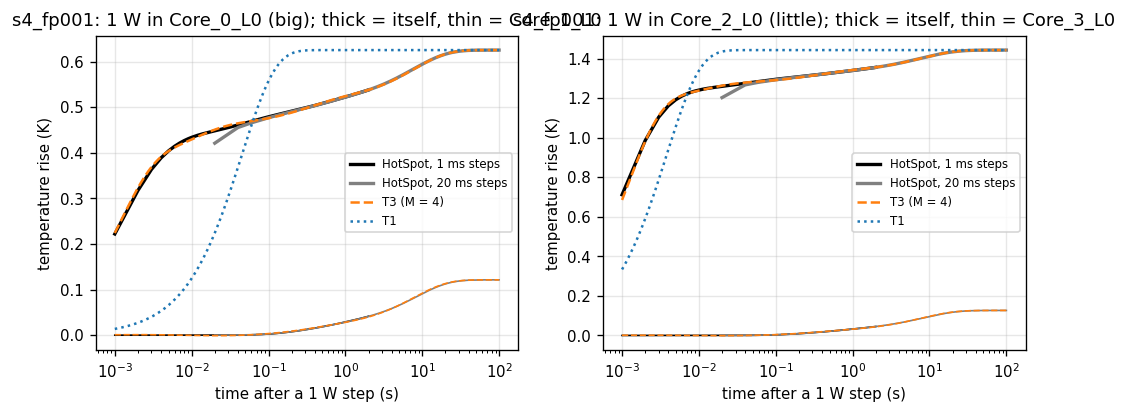
\includegraphics[width=0.9\linewidth]{P1-1_step_calibration/results/step_response_fits.png}
  \caption{Step responses to 1\,W in a big core (left) and a little core (right), log time axis.
  HotSpot (black and grey) and T3 (orange dashed) overlap; T1 (blue dotted) has the right final
  value but the wrong shape. Thin lines: coupling to a neighbouring core.}
\end{figure}

\subsection{Calibration from one long trace (ARX)}
Instead of planned steps, we recorded one long HotSpot trace with random power changes and fitted
ARX models (T2): the next rise is a linear mix of the last few rises and powers, fitted by
least squares with the steady gain constrained to $G$. Tested open loop on unseen 10\,s traces:

\begin{center}
\small
\begin{tabular}{@{}l c c c c@{}}
\toprule
Model (mean / worst) & 1\,s trace & 5\,s & 20\,s & 60\,s \\
\midrule
ARX (2,2), all blocks & 9.5 / 79\,K & 0.31 / 1.2\,K & 0.21 / 1.03\,K & 0.32 / 1.3\,K \\
ARX (3,3), all blocks & 5.2 / 67\,K & unstable & unstable & unstable \\
ARX (3,3), cores only & 4.6 / 51\,K & 0.40 / 1.5\,K & 0.32 / 0.95\,K & 0.39 / 0.96\,K \\
T3 $M=4$ from step runs & \multicolumn{4}{c}{0.062 / 0.31\,K} \\
\bottomrule
\end{tabular}
\end{center}
A trace must be at least about 5\,s long, or the slow heat sink is never seen. Beyond about 20\,s
the error rises again. Our diagnosis: least squares minimises the one-step error, which is flat
across trace lengths, while the test runs open loop for 10{,}000 steps; a pole very close to 1
turns tiny coefficient changes into tenths of a kelvin. Too many lags can make ARX unstable. T3
from planned steps is 3--5$\times$ more accurate and stable by construction.

%=====================================================================
\section{Transient predictor}

\subsection{Following HotSpot over time}
Tested from a cold chip on 2\,s traces on all 24 floorplans, 10\,s traces on four main floorplans,
and a real workload (HotSpot's EV6 floorplan with a gcc power trace).

\begin{center}
\small
\begin{tabular}{@{}l c c c c@{}}
\toprule
Model & Mean error & Worst error & Time per step & Size \\
\midrule
T1 & 7.25\,K & 14.6\,K & 1.5\us & 1.0\,kB \\
T3, $M=2$ & 0.92\,K & 2.9\,K & 3.0\us & 1.9\,kB \\
T3, $M=3$ & 0.19\,K & 1.1\,K & 3.0\us & 2.8\,kB \\
T3, $M=4$ & 0.090\,K & 0.30\,K & 3.1\us & 3.7\,kB \\
T3, $M=6$ & 0.0093\,K & 0.13\,K & 3.2\us & 5.6\,kB \\
T2 ARX (main 4 floorplans) & 0.19\,K & 0.57\,K & 5.4\us & 6.2\,kB \\
T3 $M=4$ on EV6 + gcc & 0.073\,K & 0.21\,K & 4.4\us & 28.8\,kB \\
\bottomrule
\end{tabular}
\end{center}
$M$ is the accuracy-versus-size knob; speed barely changes with it.

\subsection{Forecasting from sensor readings}
For DTM, the controller knows the current sensor readings and its planned power, and wants the
temperature some steps ahead. ``Anchored'' T3 shifts its forecast by the current difference
between sensor and model. Mean error over 352 forecast points per trace:

\begin{center}
\small
\begin{tabular}{@{}l c c c c@{}}
\toprule
Model & 1\,ms ahead & 10\,ms & 100\,ms & 1\,s \\
\midrule
No model (persistence) & 0.013\,K & 0.11\,K & 0.69\,K & 2.7\,K \\
T1 from sensors & 0.88\,K & 3.6\,K & 4.7\,K & 4.2\,K \\
T3 open loop & 0.06\,K & 0.06\,K & 0.06\,K & 0.06\,K \\
T3 anchored on sensors & 0.0009\,K & 0.0044\,K & 0.017\,K & 0.055\,K \\
T2 ARX from sensors & 0.0013\,K & 0.015\,K & 0.10\,K & 0.42\,K \\
\bottomrule
\end{tabular}
\end{center}
Persistence looks fine on average but is up to 8\,K wrong 10\,ms ahead, exactly when a power step
arrives. Anchored T3 is the best forecaster from 10\,ms to 1\,s.

\begin{figure}[H]
  \centering
  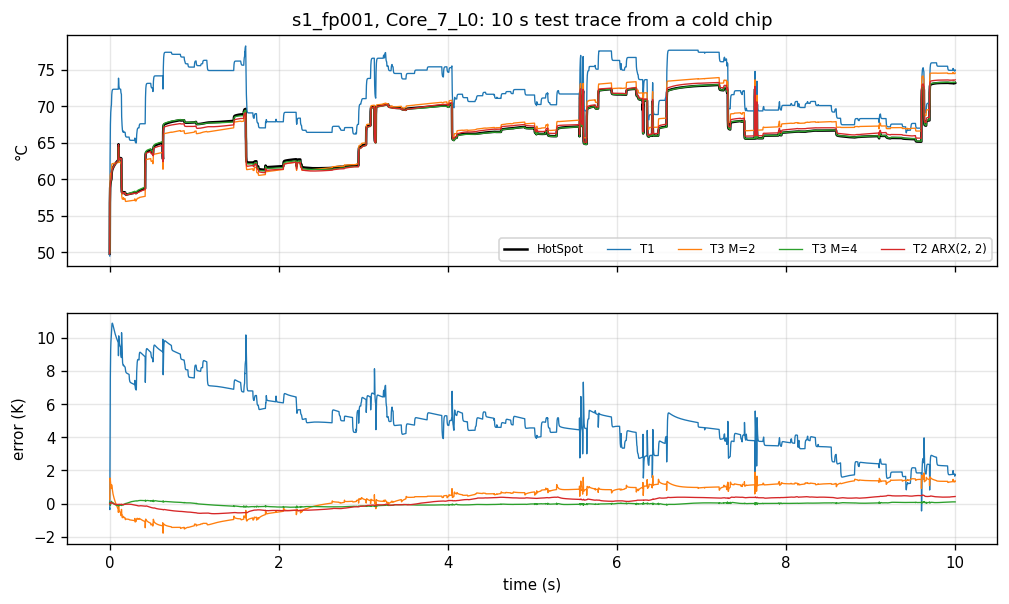
\includegraphics[width=0.48\linewidth]{P3-1_transient_predictor/results/trace_example.png}\hfill
  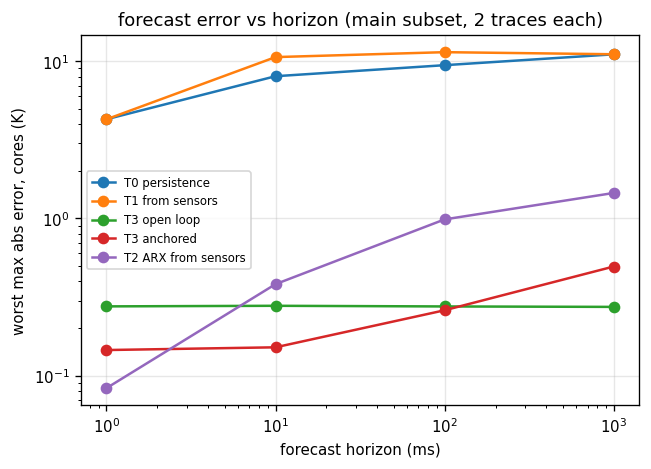
\includegraphics[width=0.48\linewidth]{P3-2_forecast_horizon/results/error_vs_horizon.png}
  \caption{Left: HotSpot and the models on one test trace; T3 sits on top of HotSpot.
  Right: forecast error against horizon.}
\end{figure}

\subsection{Trade-offs and the exact model}
Collecting every model's size, worst error and speed in one plot: in steady state S1 is exact at
464\,B, so there is no trade-off. In the transient case T3 is the Pareto front from 2 to 6\,kB;
each extra time constant costs about 1\,kB and divides the worst error by 2--4.

As an independent reference (T4), a debug patch makes HotSpot export its internal network (16{,}396
nodes). It reproduces HotSpot to $10^{-6}$\,K and its steady gain equals our calibrated $G$, which
confirms S1 independently. Model-order reduction (modal truncation, balanced truncation, and a
small filter for the dropped fast modes) gives 0.047\,K worst error with 32 states (16\,kB).
Without the fast-mode filter the error stalled at 3.3\,K for every size.

\begin{figure}[H]
  \centering
  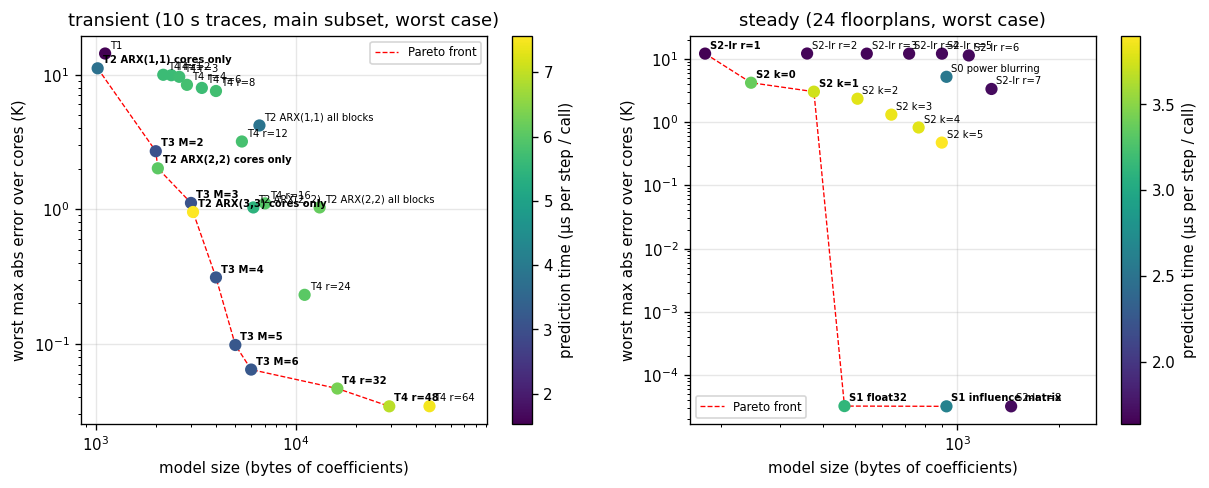
\includegraphics[width=0.48\linewidth]{P3-3_pareto/results/pareto.png}\hfill
  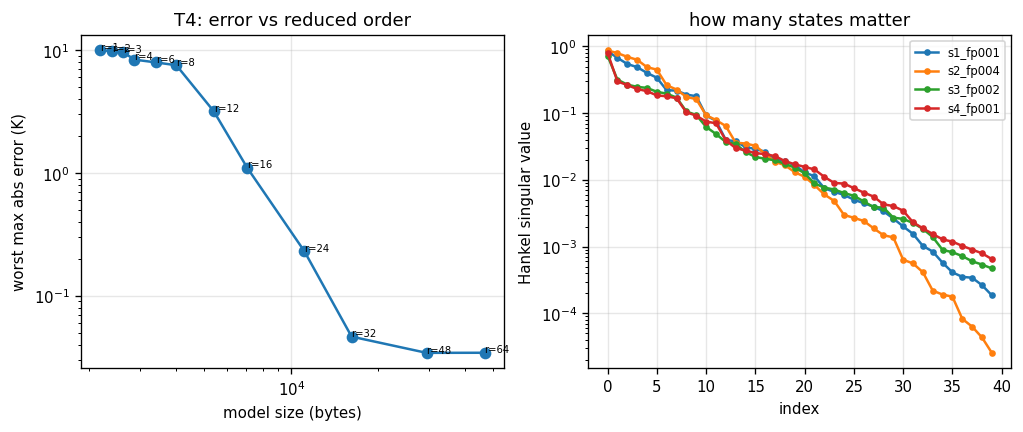
\includegraphics[width=0.48\linewidth]{P3-4_state_space_T4/results/t4_reduction.png}
  \caption{Left: size against worst error for every model; Pareto front in bold.
  Right: T4 error against the number of states.}
\end{figure}

%=====================================================================
\section{The final models and their validation on 52 new floorplans}

\subsection{Steady state: S1, with S1-hot-max for the peak}
The steady model is the influence matrix S1, $T = T_\text{amb} + G\,P$, with $G$ measured by 8
HotSpot runs of 1\,W in one core each (Stage 2). We chose it because:
\begin{itemize}
  \item \textbf{It is exact.} HotSpot is linear without leakage, so $G$ reproduces it to its
        6-decimal output (0.00003\,K worst on 7{,}248 test runs) and always picks the right
        hottest core.
  \item \textbf{It is the cheapest possible model.} 8 calibration runs (about 4\,s), one
        matrix--vector product per prediction (2.6\us), and under 1\,kB per floorplan.
  \item \textbf{There is nothing to tune.} $G$ is measured, not fitted, so it cannot overfit.
        Every calibration-free alternative was 0.5--2.7\,K off on average.
\end{itemize}
Because a core's average hides its hottest point, S1 ships together with S1-hot-max, which
predicts the hottest grid cell of each core from the same 8 runs (exact in full, about 3\,kB when
compressed).

\subsection{Transient: T3 with four time constants}
The transient model is T3 with $M=4$ (Equations~\eqref{eq:t3} and \eqref{eq:t3run}). We compared
four families and chose T3 because:
\begin{itemize}
  \item \textbf{It is accurate enough with room to spare:} 0.06--0.09\,K mean and 0.30\,K worst
        error, against targets of 0.5\,K and 1\,K, at 3.1\us\ per step and 3.7\,kB.
  \item \textbf{It is exact in steady state and stable by construction.} The weights of every pair
        sum to $G_{ij}$, so T3 agrees with S1 once power stops changing, and every filter has a
        decay factor $0 < \lambda_m < 1$, so it cannot blow up. ARX has neither guarantee: three
        lags made it unstable.
  \item \textbf{It needs only HotSpot's outputs.} The 24 calibration runs treat HotSpot as a black
        box, so the method would work with another simulator or with measurements. T4 is more
        accurate below 0.05\,K, but needs HotSpot's internal matrices and 4$\times$ the memory.
  \item \textbf{It is the best accuracy per byte} (the Pareto front from 2 to 6\,kB), and
        $M$ is a single knob: $M=6$ gives 0.13\,K worst for 5.6\,kB if more accuracy is needed.
  \item \textbf{It is the best forecaster for DTM} when anchored on the sensors, from 10\,ms to 1\,s
        ahead.
\end{itemize}
T1 was ruled out because one time constant cannot cover 1\,ms to 8\,s (14\,K worst), and ARX
because it is 2$\times$ less accurate open loop, needs a long recorded trace, and can be unstable.

\subsection{Testing on 52 generated floorplans}
The models were developed and evaluated on the 23 given floorplans. To check that these were not a
lucky set, we tested both final models on floorplans they had never seen:
\begin{itemize}
  \item \textbf{Floorplans.} Our generator produced 13 floorplans in each of the four given styles
        (52 in total), with the same cores (2 big, 6 little), the same file format and layer
        stack, and placement rules that imitate each style. Two of them turned out to be rotated
        copies of given floorplans; they were kept.
  \item \textbf{Calibration.} Each floorplan was calibrated from scratch exactly as a new user would
        do it: 8 steady runs for S1 and all 24 runs for T3 ($M=4$).
  \item \textbf{Tests.} S1 on 302 steady power vectors per floorplan (nominal, maximum and 300
        random); T3 on a 2\,s phase trace from a cold chip, in which every core switches between
        power levels in phases of 1\,ms to 2\,s. None of these inputs is used in calibration.
        Everything ran on one laptop in about 100 minutes.
\end{itemize}

\begin{center}
\small
\begin{tabular}{@{}l c c c c c@{}}
\toprule
Style & Floorplans & S1 mean & S1 worst & T3 mean & T3 worst \\
\midrule
Style 1 & 13 & $6.8\times10^{-6}$\,K & $3.4\times10^{-5}$\,K & 0.108\,K & 0.34\,K \\
Style 2 & 13 & $6.7\times10^{-6}$\,K & $2.6\times10^{-5}$\,K & 0.114\,K & 0.32\,K \\
Style 3 & 13 & $6.6\times10^{-6}$\,K & $2.8\times10^{-5}$\,K & 0.085\,K & 0.31\,K \\
Style 4 & 13 & $6.1\times10^{-6}$\,K & $2.6\times10^{-5}$\,K & 0.056\,K & 0.26\,K \\
All generated & 52 & $6.5\times10^{-6}$\,K & $3.4\times10^{-5}$\,K & 0.091\,K & 0.34\,K \\
Given floorplans & 24 & $6\times10^{-6}$\,K & $3\times10^{-5}$\,K & 0.090\,K & 0.30\,K \\
\bottomrule
\end{tabular}
\end{center}

\begin{figure}[H]
  \centering
  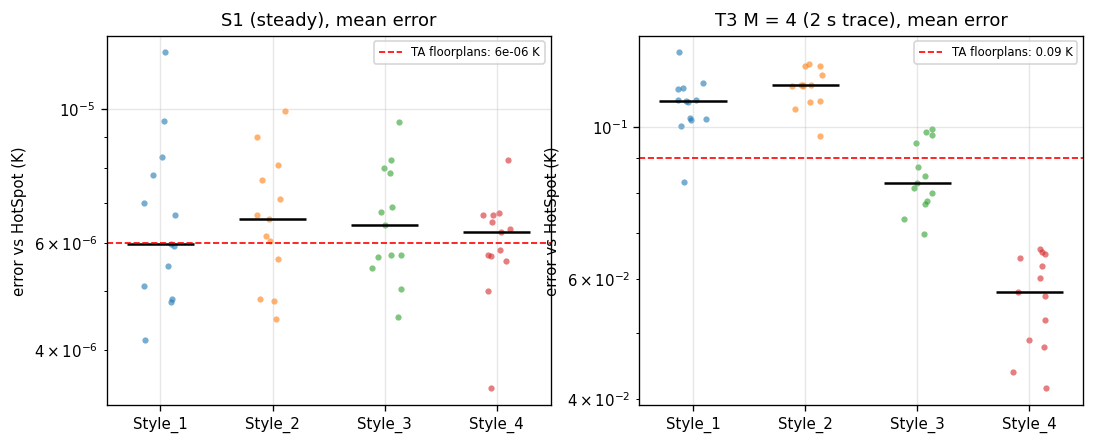
\includegraphics[width=0.48\linewidth]{extended_validation/results/error_by_style.png}\hfill
  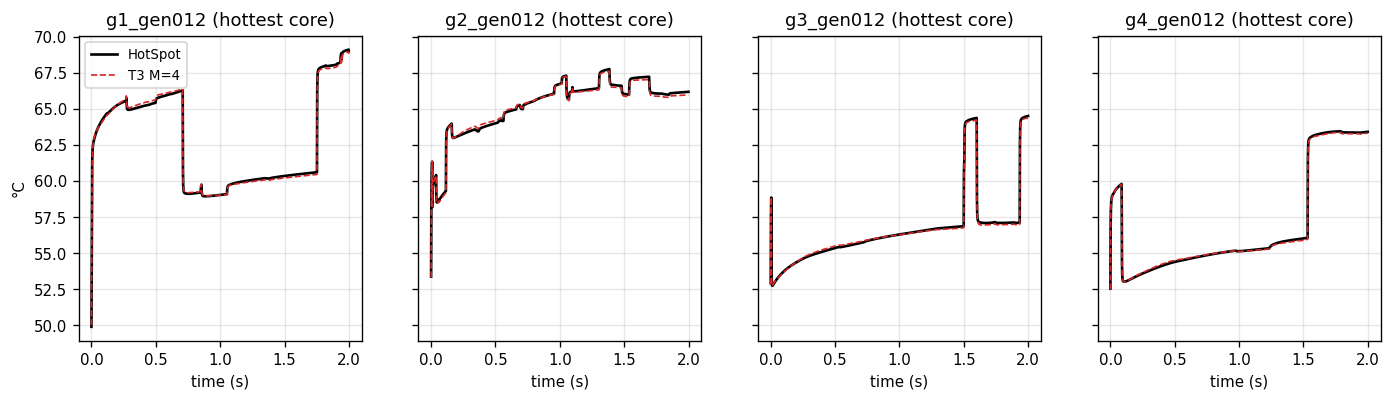
\includegraphics[width=0.48\linewidth]{extended_validation/results/transient_check.png}
  \caption{Left: one dot per generated floorplan, black bar = median, red line = given floorplans.
  Right: the hottest core on a test trace; T3 (red dashed) follows HotSpot (black).}
\end{figure}

\begin{figure}[H]
  \centering
  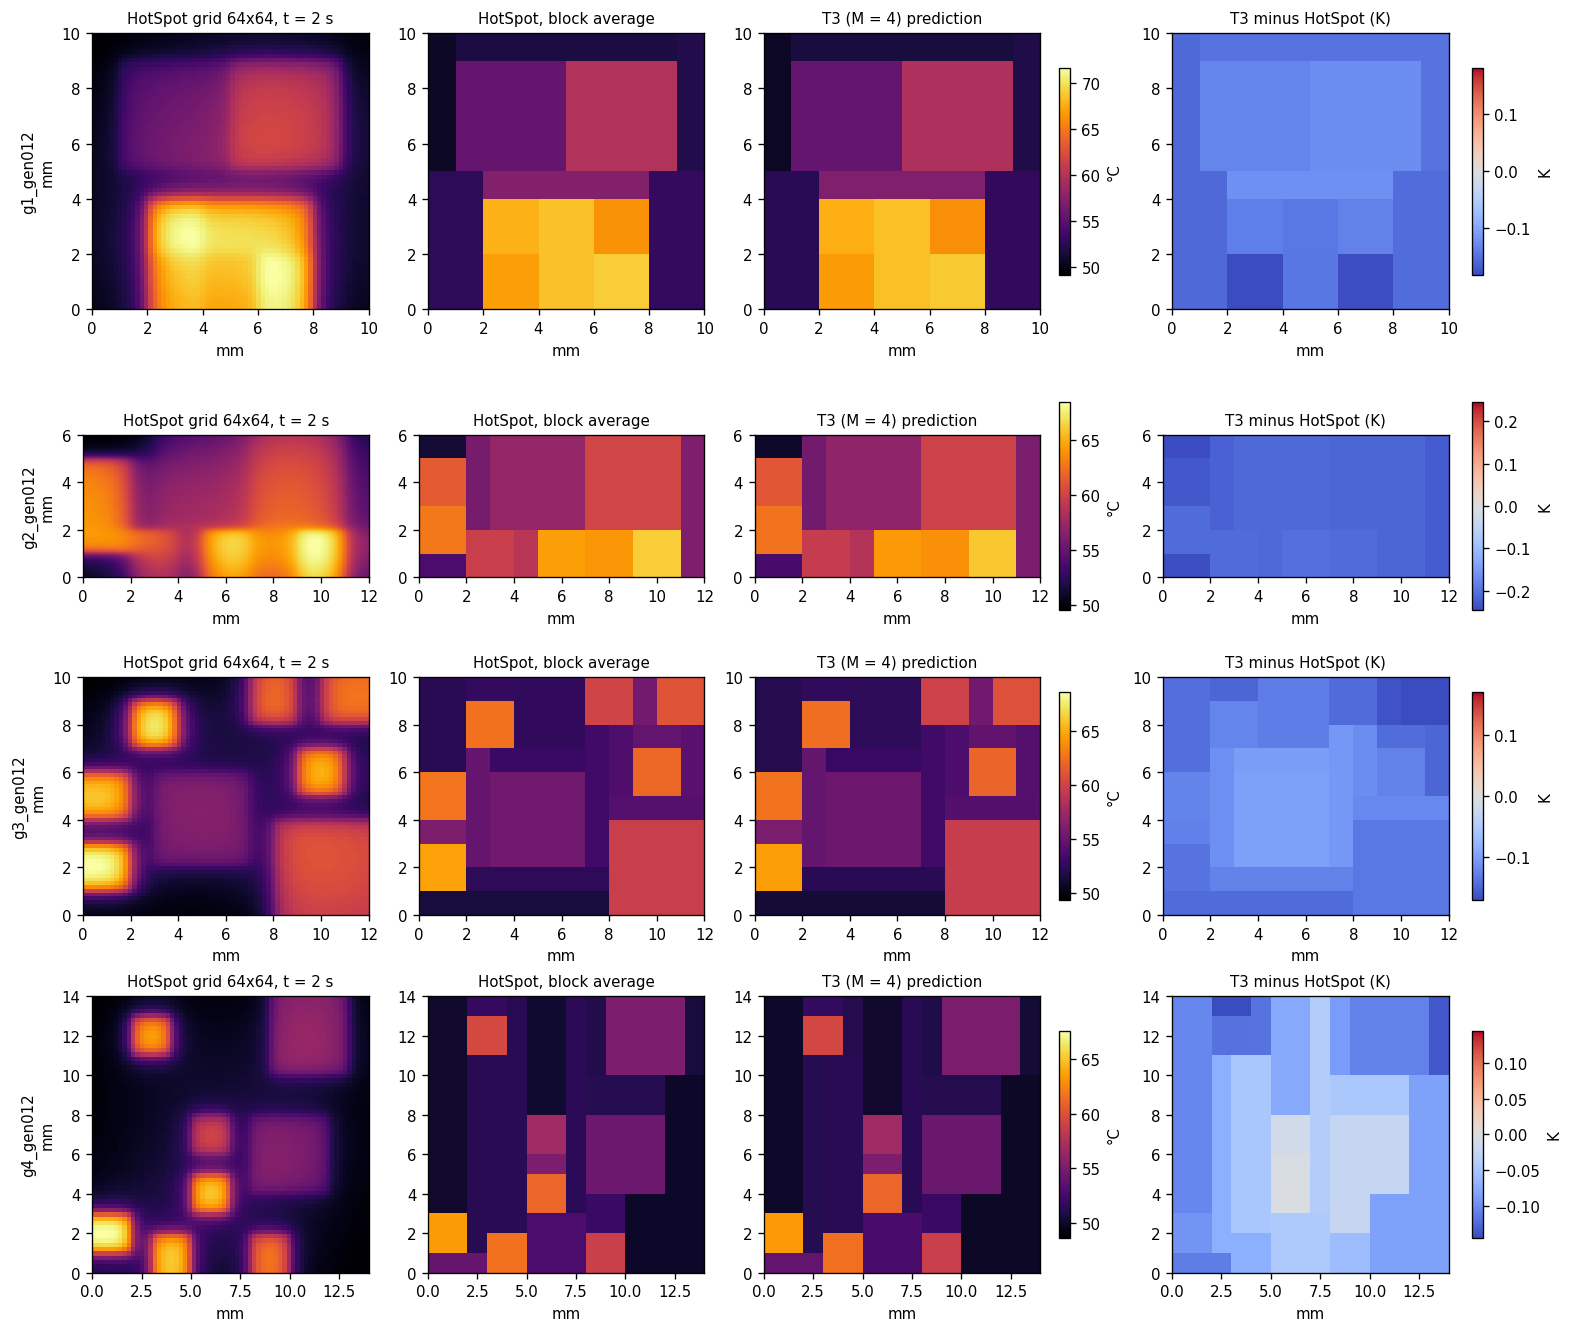
\includegraphics[width=\linewidth]{extended_validation/results/heatmaps_t3.png}
  \caption{T3 at the end of the 2\,s test trace, one generated floorplan per style. Columns:
  HotSpot's $64\times64$ map; HotSpot's block averages; T3's prediction (same colour scale); T3
  minus HotSpot in kelvin.}
\end{figure}

\begin{itemize}
  \item \textbf{The results carry over.} Over 52 new floorplans, S1 is off by about 0.000007\,K and
        T3 by 0.09\,K on average, the same as on the given floorplans. Nothing broke on any
        floorplan.
  \item \textbf{S1 is independent of the floorplan.} Its error is at HotSpot's rounding and it picks
        the hottest core correctly on every floorplan.
  \item \textbf{T3 varies a little with style}, from 0.056\,K (Style 4) to 0.114\,K (Style 2); the
        spread within a style is about as large as between styles. It names the right hottest
        core in 88--100\,\% of steps; misses happen when two cores are within a fraction of a
        kelvin.
  \item \textbf{T3's map matches HotSpot's} within 0.14--0.25\,K in every block at $t = 2$\,s. It
        was slightly too cool in every block at that moment (by 0.09--0.21\,K for the hottest
        core), so a thermal limit needs a margin of a few tenths of a kelvin.
\end{itemize}

%=====================================================================
\section{Robustness}

\subsection{Unusual inputs}
\begin{center}
\small
\begin{tabular}{@{}l c c l@{}}
\toprule
Case (4 main floorplans) & T3 mean & T3 worst & Verdict \\
\midrule
Normal trace (reference) & 0.10\,K & 0.32\,K & fine \\
Steady power at 3$\times$ the maximum (S1) & 0.00002\,K & 0.00005\,K & fine \\
Transient at 2$\times$ power & 0.21\,K & 0.64\,K & fine (1\,\% of rise) \\
Bursty power, switching every 1--5\,ms & 0.11\,K & 0.44\,K & fine \\
Task migration between cores & 0.076\,K & 0.31\,K & fine \\
Time step 0.1\,ms instead of 1\,ms & 0.14\,K & 2.16\,K & weak spot \\
Time step 10\,ms & 0.079\,K & 1.88\,K & weak spot \\
Warm start (after the first 50\,ms) & 0.029\,K & 0.27\,K & fine \\
\bottomrule
\end{tabular}
\end{center}
The coefficients describe the chip, not the workload, so power level, burstiness and task
placement do not matter. A different time step does (1--2\,K worst); the fix is to calibrate at
the time step the DTM controller uses.

\subsection{Package changes}
The coefficients belong to one floorplan \emph{and} one package. We changed the package in three
ways on two floorplans (s1\_fp001 and s4\_fp001), one change at a time: ambient 35\degC\ instead of
45\degC; heat-sink convection resistance doubled (0.1 to 0.2\,K/W, a worse cooler); and halved
(0.05\,K/W, a better cooler). Under each new package we tested the old models (S1 and T3, $M=4$)
and models recalibrated with the usual 24 runs, on 50 random steady vectors and a 3\,s trace from
a cold chip.

\begin{center}
\small
\begin{tabular}{@{}l l c c@{}}
\toprule
Change & Model & Steady worst & Transient worst (3\,s) \\
\midrule
Ambient 35\degC & old model, old $T_\text{amb}$ & 10.0\,K & 10.2\,K \\
 & old model, new $T_\text{amb}$ & 0.00001--0.00002\,K & 0.23--0.27\,K \\
 & recalibrated & 0.00001--0.00002\,K & 0.23--0.27\,K \\
\midrule
Convection resistance $\times 2$ & old model & 8.5\,K & 0.43--0.48\,K \\
 & recalibrated & 0.00001--0.00002\,K & 0.26--0.29\,K \\
\midrule
Convection resistance $\times 0.5$ & old model & 4.4\,K & 0.42--0.48\,K \\
 & recalibrated & 0.00002\,K & 0.20--0.22\,K \\
\bottomrule
\end{tabular}
\end{center}
\begin{itemize}
  \item \textbf{A new ambient needs no recalibration.} The models predict the rise above ambient,
        so the old coefficients with the new $T_\text{amb}$ give exactly the same errors as
        recalibrated ones. Forgetting to update $T_\text{amb}$ is a 10\,K error.
  \item \textbf{A new heat sink needs recalibration.} The old coefficients are 8.5\,K off in steady
        state when the convection resistance doubles and 4.4\,K when it halves; 24 runs under the
        new package bring the error back to $10^{-5}$\,K.
  \item \textbf{The error appears slowly in transients.} Over a 3\,s trace the old model is only
        0.4--0.5\,K off, because the heat sink takes tens of seconds to warm up. After a long run
        the full steady error applies, so a DTM controller would drift.
  \item \textbf{The error is almost exactly the change in resistance times the total power}
        (0.1\,K/W $\times$ about 85\,W $\approx$ 8.5\,K; 0.05\,K/W $\times$ about 87\,W
        $\approx$ 4.4\,K), the same on both floorplans. A sink change therefore mainly adds the same
        amount to every entry of $G$, which suggests it could be corrected without HotSpot runs.
\end{itemize}

\subsection{Leakage}
Real chips leak more power when hot, which breaks linearity. HotSpot's leakage model (steady state
only) makes every block of the silicon layer, white space included, leak
\begin{equation}
  P_{\text{leak},i}(T_i) = \alpha\, A_i\, e^{\beta\,(T_i - 383.15\,\text{K})},
  \qquad \alpha = 1.5\times10^{4}\,\text{W/m}^2,\ \beta = 0.036\,\text{K}^{-1},
  \label{eq:leak}
\end{equation}
where $A_i$ is the block's area, and iterates power and temperature until they settle. At our
temperatures this is small (0.2--0.5\,W per chip), so we also built a HotSpot with 10$\times$
$\alpha$ (2--5\,W, 3--5\,\% of chip power). Test: four main floorplans, 50 random power vectors
each, in both builds.

\textbf{The fix to S1.} The chip is still linear in the \emph{total} power, so the calibrated
coefficients stay valid; only the leakage has to be added as extra power. Since the white-space
blocks leak too, $G$ is extended to $G_\text{all}$, with one column for every block of the silicon
layer (one extra steady run per white-space block, 3--17 runs). Starting from the plain S1
prediction $T^{(0)} = T_\text{amb} + G\,P$, the loop repeats
\begin{equation}
  T^{(k+1)} = T_\text{amb} + G_\text{all}\left(P + P_\text{leak}\big(T^{(k)}\big)\right)
  \label{eq:leakloop}
\end{equation}
until the temperatures change by less than $10^{-4}$\,K. The leakage formula (\ref{eq:leak}) is
assumed known, since it belongs to the technology, not the floorplan.

\begin{center}
\small
\begin{tabular}{@{}l c c c c c@{}}
\toprule
Leakage & Leakage power & S1 alone (worst) & S1 + loop (worst) & Iterations & Time \\
\midrule
Default & 0.2--0.5\,W & 0.08--0.10\,K & $1$--$2\times10^{-5}$\,K & 3 & 22--25\us \\
10$\times$ stronger & 2--5\,W & 0.77--1.07\,K & $2$--$6\times10^{-5}$\,K & 4 & 29--33\us \\
\bottomrule
\end{tabular}
\end{center}
Ignoring leakage costs about 0.1\,K at default strength and 1\,K at 10$\times$. The loop removes
the error completely, back to HotSpot's output precision, in 3--4 iterations; it is about
10$\times$ slower than S1 alone but still about 10{,}000$\times$ faster than one HotSpot run.
HotSpot does not support leakage in transient runs, so the transient side could not be tested;
the same loop would apply to T3 at each time step. Most of the leakage comes from the white space,
so these numbers are an upper bound if the white space is empty silicon.

%=====================================================================
\section{The tool: \texttt{ltp}}
Both stages are available as commands that need only NumPy and a model file:
{\small\begin{verbatim}
python3 -m src.ltp calibrate s4_fp001 -o model_s4_fp001.npz
python3 -m src.ltp steady    model_s4_fp001.npz --power 20,20,8,8,8,8,8,8
python3 -m src.ltp transient model_s4_fp001.npz --ptrace trace.ptrace -o out.ttrace
python3 -m src.ltp forecast  model_s4_fp001.npz --history past.ptrace \
                             --temps T_now.txt --next plan.ptrace
python3 -m src.ltp bench     model_s4_fp001.npz s4_fp001
\end{verbatim}}
The given \texttt{.ptrace} files are read directly, and transient output is a HotSpot-style
\texttt{.ttrace}. Output of \texttt{bench} on s4\_fp001: model 8{,}032\,B; steady error
$5.2\times10^{-6}$\,K mean and $1.4\times10^{-5}$\,K max at 2.6\us\ per call; transient error
0.051\,K mean and 0.189\,K max at 3.5\us\ per step. Seven unit tests pass.

%=====================================================================
\section{What went as planned, and what deviated}
\textbf{As planned:} the two-stage design; HotSpot grid model as the reference; S1 as the steady
model with 8 runs; T3 as the transient model; evaluation on accuracy, time and size; the
calibration-is-needed check; robustness studies; the \texttt{ltp} tool. All steady and transient
targets were met, except calibration wall time (about 2.75\,min per floorplan against a target of
2\,min).

\begin{center}
\small
\begin{tabular}{@{}p{3cm} p{4.3cm} p{7.7cm}@{}}
\toprule
Item & Planned & Done, and why \\
\midrule
HotSpot build & Precision patch & Also LU caching (29$\times$ faster) and a memory-leak fix: a 60\,s trace took 4\,h or ran out of memory. \\
Dataset & Our synthetic floorplans & The 23 given floorplans as the main set, plus 52 generated in the same styles. \\
Hot spots & One hottest cell per core & S1-hot-max over all cells of a core, which is exact, compressed by dropping cells that can never be the hottest. \\
\bottomrule
\end{tabular}
\end{center}

%=====================================================================
\section{Pending items (for Stage 4)}
\begin{itemize}
  \item Report the proactive DTM results (closed-loop HotSpot, reactive vs proactive DTM, core
        placement).
  \item Re-measure all timings on an idle machine.
  \item Package \texttt{ltp} for \texttt{pip install}.
  \item Final report, code archive, README with run instructions, and presentation feedback.
  \item Open questions about the given dataset (HotSpot configuration used, Style 2 power files,
        meaning of the FILL white space for leakage).
\end{itemize}

%=====================================================================
\section{Learnings}
\begin{enumerate}
  \item HotSpot is linear without leakage, so a matrix predictor can be exact, not approximate.
  \item Calibration is cheap and essential: 8 runs (4\,s) make the steady model exact; skipping it
        costs 0.5--2.7\,K on average and up to 12\,K.
  \item Position on the die matters, not just core type: edges, neighbours and die size make each
        floorplan's coefficients unique.
  \item Little cores are the hot ones: higher power density means about 2.4$\times$ the
        self-heating per watt.
  \item Core averages hide hot spots 3--9\,K hotter, and the hot spot moves.
  \item Heat moves on time scales from 1\,ms to 8\,s; one time constant cannot capture this, four
        can.
  \item Planned step runs beat fitting a recorded trace, by 3--5$\times$ and with guaranteed
        stability.
  \item Forecasting needs a model: ``temperature stays the same'' is up to 8\,K wrong 10\,ms
        ahead.
  \item A model belongs to its cooler too: a new ambient is free, a new heat sink needs
        recalibration.
  \item Engineering the reference (precision, speed, memory) was a prerequisite for every
        experiment.
\end{enumerate}

%=====================================================================
\section{Future scope}
\begin{itemize}
  \item Correcting a heat-sink change without new HotSpot runs (the error is close to
        $\Delta R_\text{sink}\times$ total power).
  \item Leakage in transient prediction, with a simulator that supports it.
  \item Fitting ARX to the multi-step (open-loop) error instead of the one-step error.
  \item Task migration between big and little cores as a DTM action.
  \item Hot-spot models that scale to many cores.
  \item Calibration from real sensor measurements instead of a simulator; T3 and S1 only need
        input--output data, so the method carries over.
\end{itemize}

%=====================================================================
\section{LLM assistance disclosure}
LLMs were used to understand HotSpot, for literature review to select appropriate models, generate
floorplans, and calibration and testing scripts.

\end{document}
